\section{Betriebswirtschaftliche Analyse}
\subsection{Beschreibung möglicher Anwendungen aus Business-Sicht}

Um Faktoren und Kennzahlen für den langfristigen Erfolg des Unternehmens zu erstellen, können die bereitgestellten Daten des Online-Shops aus verschiedenen Perspektiven betrachtet werden. Ein mögliches Vorgehensmodell bildet hierfür die Balanced-Scorecard.

Die bedeutendste Perspektive bei Analyse der bereitgestellten Daten ist die finanzielle Sicht. Zu dieser gehören typische betriebswirtschafliche Kennzahlen wie der Gewinn, der Umsatz und die Rentabilität. Als Ziel für diese Perspektive kann die Steigerung der genannten Kennzahlen angesehen werden. Auch die Identifikation und Abstoßung unrentabler Produkte kann als Ziel für die finanzielle Perspektive betrachtet werden. Da jedoch nur die Verkaufspreise zur Verfügung stehen, beschränkt sich die Analyse auf die Umsatzentwicklung und -verteilung. Der Umsatz soll dabei in Abhängigkeit der Dimensionen Zeit, Produkt, Alter bzw. Geschlecht der Kunden betrachtet werden. Auf Basis der Ergebnisse dieser Analyse lassen sich beispielsweise die Top-Seller oder auch die kaufkräftigsten Kundengruppen bestimmen.

Eine weitere Betrachtungsweise ist die Kundenperspektive. Mögliche Ziele sind hierbei eine hohe Kundenzufriedenheit sowie ein hoher Neukundenanteil. Eine denkbare Fragestellung wäre auch, welche Produkte werden von Kunden häufig zusammen gekauft, was auch als Cross-Selling bezeichnet wird. Mithilfe dieser Analyse können für potentielle Kunden spezielle Angebote erstellt werden, um so den Umsatz pro Bestellung zu erhöhen. Daraus abgeleitete Kennzahlen sind die Bestellungen pro Kunde und Artikel pro Bestellung.

Zur Analyse und Bewertung der internen Geschäftsprozesse können die Bearbeitungszeiten der Bestellungen oder die Retouren betrachtet werden. Diese gilt es zu verringern.
So könnte bei der Anzahl der Retouren analysiert werden, ob es bei diesen einen besonders häufigen Grund gibt. Sollten bestimmte Artikel beispielsweise besonders häufig wegen mangelnder Qualität reklamiert werden, so liegt die Empfehlung nahe, diese aus dem Warenangebot zu entfernen.

Der vierte Punkt der Balanced-Scorecard wird als Lernen und Wachstum bezeichnet. Dabei geht es um die Zufriedenheit der Mitarbeiter und deren Qualifikationen. Dazu sind jedoch keine Daten vorhanden und eine Analyse daher nicht möglich.

\pagebreak

\subsection{Konzeptuelle Modellierung}

\subsubsection*{Cross-Selling}
\begin{figure}[htbp] 
  \centering
     \includepdf[pages=3,pagecommand={},scale=1.2,offset=2.5cm 2.0cm]{phase1/adapt-diagramme.pdf}
\end{figure}
\vspace{10cm}
Mithilfe dieses Cubes soll ermittelt werden, welche Produkte bzw. Produktgruppen besonders häufig zusammen gekauft werden. Auf Basis der Ergebnisse dieser Untersuchung können beispielsweise besondere Angebote oder Produktkombinationen erstellt werden, um so den Umsatz pro Bestellung zu erhöhen.
\pagebreak

\subsubsection*{Retouren}
\begin{figure}[htbp] 
  \centering
     \includepdf[pages=2,pagecommand={},scale=0.85,offset=-0.2cm 7.2cm]{phase1/adapt-diagramme.pdf}
\end{figure}
\vspace{9cm}
Der Cube \textit{Retouren} beinhaltet die Anzahl der Retouren verteilt auf die Dimensionen \textit{Rückgabegrund}, \textit{Zeit}, \textit{Produkt}, \textit{Alter} bzw.\textit{ Geschlecht} der Kunden. Darüber soll untersucht werden, welche Gründe häufig zur Retoure führen, wann gehäuft Retouren auftreten, welche Produkte zurückgegeben werden und wie sich verschiedene Kundengruppen verhalten. So können unter Umständen häufig reklamierte Produkte erkannt und aus dem Angebot entfernt werden.
\pagebreak




\subsubsection*{Bestellungen}
\begin{figure}[htbp] 
  \centering
     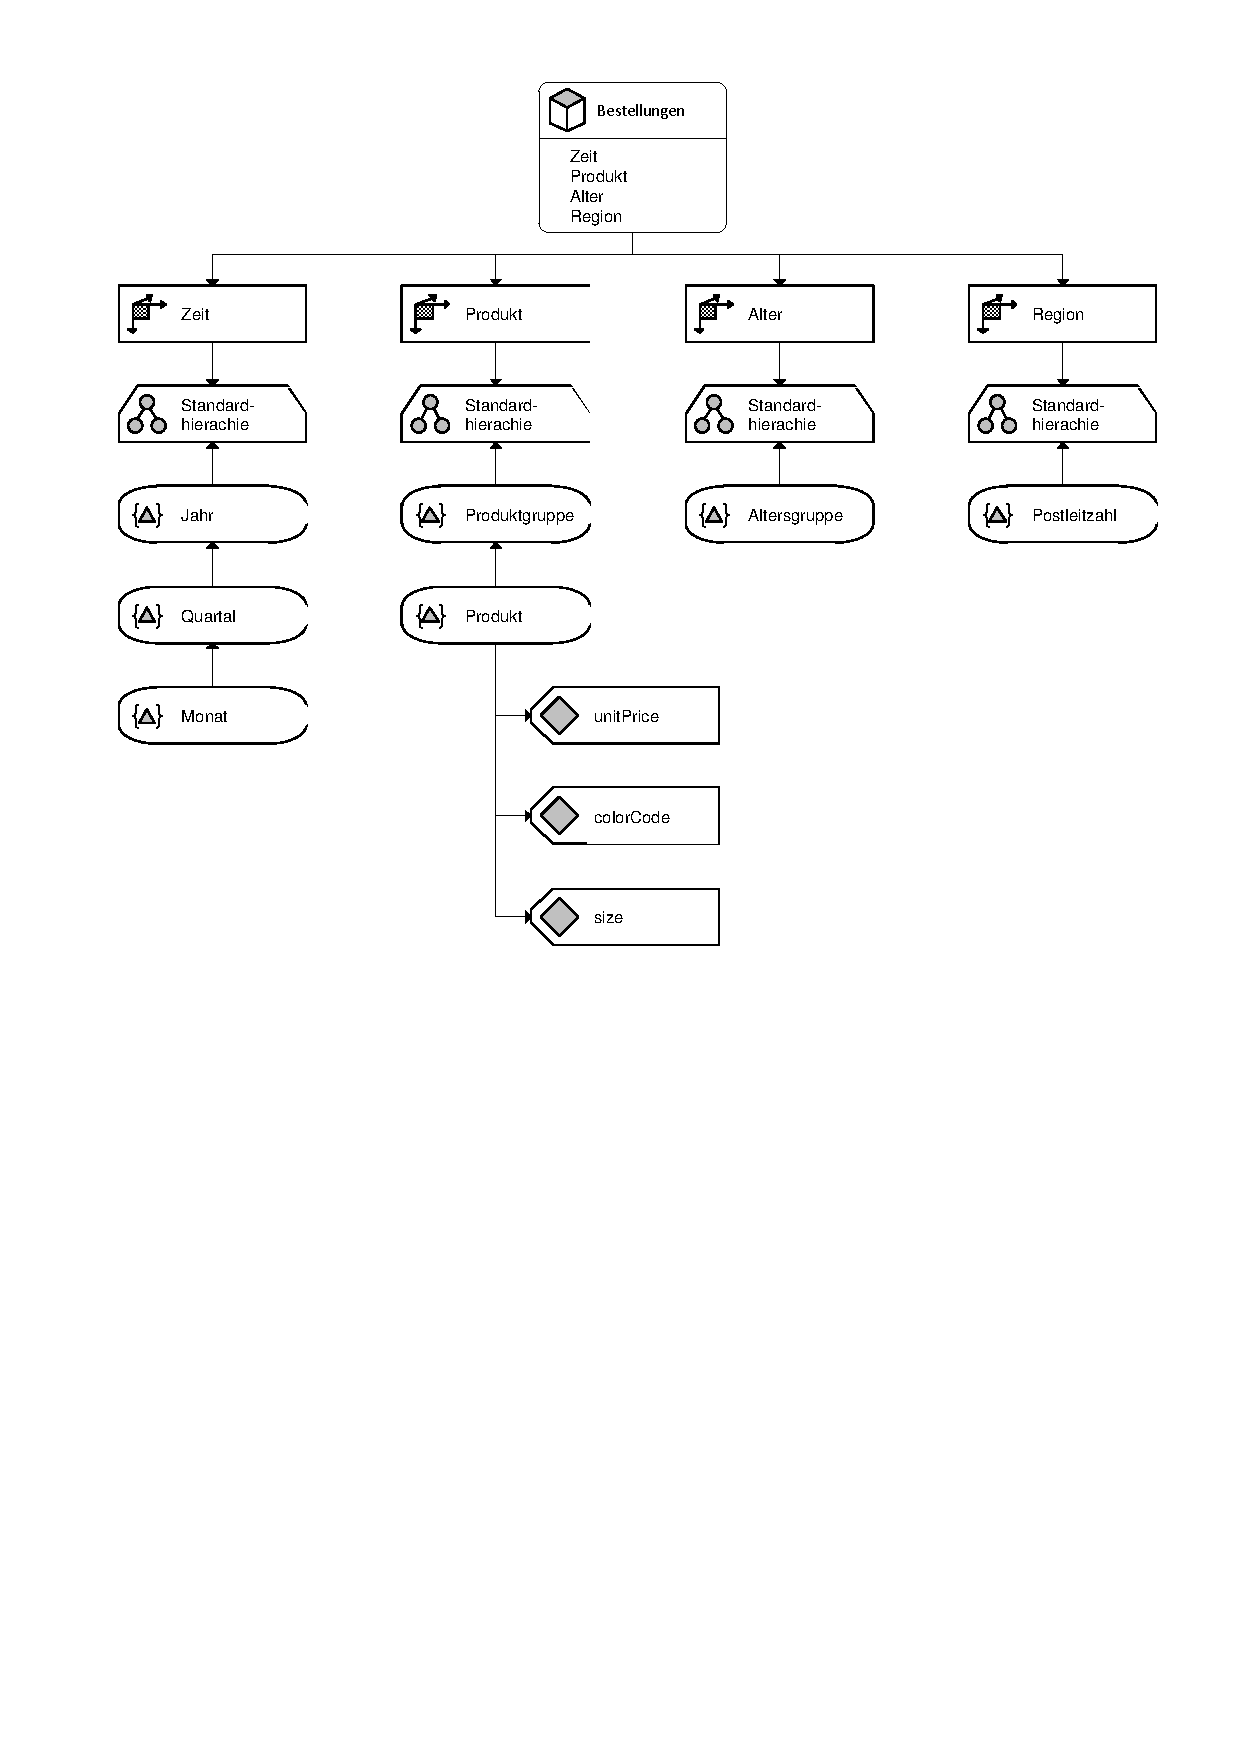
\includepdf[pages=1,pagecommand={},scale=0.85,offset=0cm 5.5cm]{phase1/adapt-diagramme.pdf}
\end{figure}
\vspace{10cm}
Mit dem Cube \textit{Bestellungen} soll die Anzahl der Bestellungen in Abhängigkeit der \textit{Zeit}, des\textit{ Produktes} sowie der Kundenattribute \textit{Alter}, \textit{Geschlecht} und \textit{Newsletter-Abonement} betrachtet werden. Mithilfe dieser Analyse lassen sich sowohl die \glqq Top-Seller\grqq ~als auch die \glqq Ladenhütter\grqq ~des Sortiments auf einfache Weise erkennen. Zusammen mit dem Verkaufspreis und der Anzahl der Retouren aus der vorherigen Untersuchung lässt sich so auch die Umsatzverteilung bezogen auf die einzelnen Produkte und Kundengruppen berechnen. Durch Dimension \textit{Newsletter} soll ermittelt werden, ob dieser einen Einfluss auf Bestellverhalten der einzelnen Kundengruppen hat.


\pagebreak

\subsection{Datenverarbeitungsanforderungen}

Da als Datenquelle die operative Datenbank des Online-Shop dient, stellt diese bezogen auf die Granularität, die Aktualität und die Glaubwürdigkeit eine ausreichend hohe Datenqualität bereit.
Für weiterführende Analysen bezüglich des Gewinns oder der Rentabilität sind die Daten der Datenbank jedoch nicht ausreichend, da Informationen über Einkaufspreise und Ähnliches nicht zur Verfügung stehen. Hierfür müssten externe Datenquellen, wie Preislisten von Großhändlern, in den Analyseprozess integriert werden.

Für das Auslesen der Basisdaten bietet sich eine periodische Extraktion an, da der Fokus bei den Analysen auf der zeitlichen Entwicklung bzw. Verteilung der festgelegten Kennzahlen liegt.
Da in der Zeit-Dimension der Monat die kleinste Konsolidierungsstufe bildet, genügt es die Datenextraktion und Auswertung ein- bis zweimal im Monat durchzuführen.
